\documentclass{standalone}
\usepackage{tikz}
\usepackage{mathtools}
\usepackage{pgfplots, pgfplotstable}

\pgfplotsset{compat = newest}

\definecolor{color1}{RGB}{255,158,1}
\definecolor{color2}{RGB}{255,74,1}
\definecolor{color3}{RGB}{220,0,0}

\begin{document}
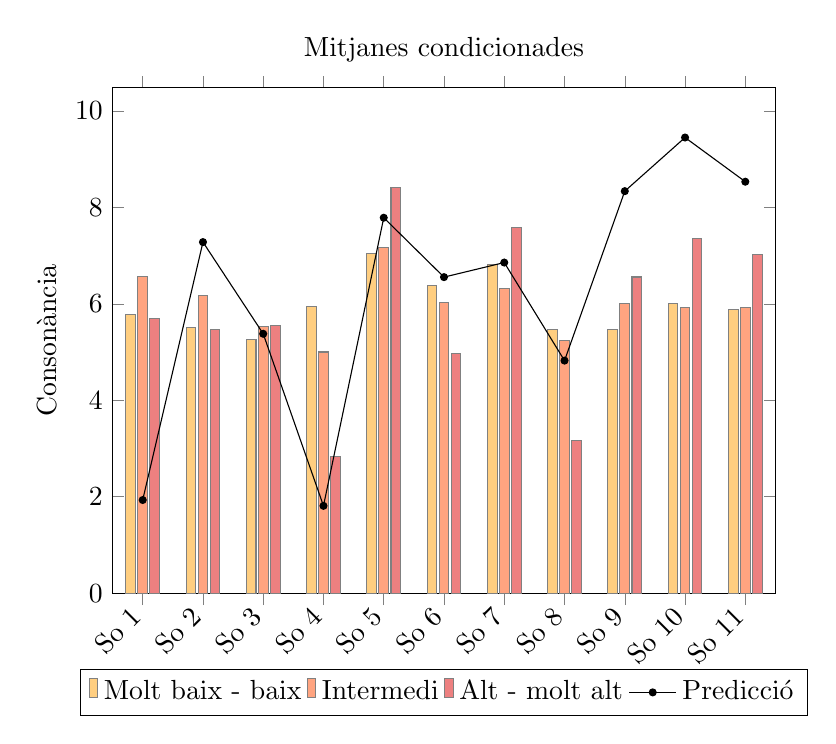
\begin{tikzpicture}
\pgfplotsset{
    /pgfplots/ybar legend/.style={
        /pgfplots/legend image code/.code={
            \draw [##1,/tikz/.cd,bar width=3pt,yshift=-0.2em,bar shift=0pt]
            plot coordinates {(0cm,0.7em)};
        },
    },
}
\begin{axis}[
    title=Mitjanes condicionades,
    ybar=0.03cm, %sets vertical columns and shift between x-axis groups of data.
    width=10cm,
    height=8cm,
    ymin=0.475,
    ymax=10,
    xmin=So 1,
    enlargelimits=0.05, %enlarge limits of the plot
    legend style={at={(0.5,-0.15)},
    anchor=north,legend columns=-1},
    x tick label style={rotate=45,anchor=east},
    ylabel={Consonància},
    symbolic x coords={So 1,So 2,So 3,So 4,So 5,So 6,So 7,So 8,So 9,So 10,So 11},
    xtick=data,
    % nodes near coords,
    % nodes near coords align={vertical},
    bar width=3.5pt,
    ]
\addplot[black!50,fill=color1!50] coordinates {
(So 1,5.784)
(So 2,5.505)
(So 3,5.252)
(So 4,5.937)
(So 5,7.036)
(So 6,6.387)
(So 7,6.811)
(So 8,5.468)
(So 9,5.468)
(So 10,6.009)
(So 11,5.874)};
\addplot[black!50,fill=color2!50] coordinates {
(So 1,6.558)
(So 2,6.163)
(So 3,5.535)
(So 4,5)
(So 5,7.163)
(So 6,6.023)
(So 7,6.326)
(So 8,5.233)
(So 9,6)
(So 10,5.93)
(So 11,5.93)};
\addplot[black!50,fill=color3!50] coordinates {
(So 1,5.694)
(So 2,5.472)
(So 3,5.556)
(So 4,2.833)
(So 5,8.417)
(So 6,4.972)
(So 7,7.583)
(So 8,3.167)
(So 9,6.556)
(So 10,7.361)
(So 11,7.028)};
\addplot[line legend,thin,mark=otimes*,sharp plot,black,mark size=1.25pt] coordinates {
(So 1,1.932)
(So 2,7.279)
(So 3,5.378)
(So 4,1.811)
(So 5,7.784)
(So 6,6.553)
(So 7,6.855)
(So 8,4.822)
(So 9,8.335)
(So 10,9.447)
(So 11,8.531)}; %Some available options inside [...]: mark=square*,otimes*,triangle*,diamond*,*,square*,otimes*,star,diamond*
\legend{Molt baix - baix,Intermedi,Alt - molt alt,Predicció}
\end{axis}
\end{tikzpicture}
\end{document}
